% Define margins
\voffset=-1in
\hoffset=-1in

% A4
\headheight=4ex
\headsep=2ex

\evensidemargin=2.5cm
\oddsidemargin=2.5cm
%\topmargin=1.3cm
\topmargin=0.0cm
\marginparwidth=1.5cm

\textwidth=16.0cm
\textheight=23.9cm

\footskip=6ex
\parindent=0cm
\parskip=1ex

\newlength{\mmntboxwidth}
\setlength{\mmntboxwidth}{\textwidth}
\addtolength{\mmntboxwidth}{-2mm}

\setcounter{secnumdepth}{4}
\setcounter{tocdepth}{2}

\shortindexingoff
%\newindex{idxkey}{idxkey}{indkey}{Index of Keywords}
%\newindex{idxipd}{idxipd}{indipd}{Index of Material Parameters}
\makeindex

\newcommand{\auxindex}[1]{\index{auxiliary tools!#1@\texttt{#1}}%
\index{#1@\texttt{#1}}}

\newlength{\NoteBoxWidth}
\setlength{\NoteBoxWidth}{14.5cm}%{15.18cm}
\newrgbcolor{notebg}         {0.99609375 0.8828125 0.921875}  % PSTricks colors
\newrgbcolor{tipbg}          {0.98828125 0.99609375 0.78515625}
\newrgbcolor{ipdbg}          {0.85  0.85  0.93}
\definecolor{headingfg} {rgb}{0.2,0.2,0.6}  
\newrgbcolor{headingfg}      {0.2 0.2 0.6}  % PSTricks colors

\newlength{\IpdBoxWidth}
\setlength{\IpdBoxWidth}{14.5cm}

\newcommand{\verbbaseformat}[2] {\psframebox*[boxsep=false,fillcolor=#1]{
                                 %\parbox{\IpdBoxWidth}{\color{black}#2\raisebox{-1ex}{\rule{0pt}{2.6ex}}}}}
                                 \parbox{\IpdBoxWidth}{\color{black}#2\raisebox{-1.5ex}{\rule{0pt}{2.6ex}}}}}
\newcommand{\verbformat}[1]     {\verbbaseformat{\verbatimbg}{#1}}
\newcommand{\verbatimbg}        {ipdbg}
\renewcommand{\FancyVerbFormatLine}[1]{\verbformat{#1}}

\newcommand{\EXA}{}
\newcommand{\mmntcaparg}{}
\newcommand{\mmntlabarg}{}
\newcommand{\stdin}[1]{\texttt{#1}}
\newcommand{\unit}[1]{$\mathrm{#1}$}

\makeatletter % [JW] check latex faq for : \@ and @ in macro names
\newcommand{\mmnttablecaption}[1]{%
\par
\addcontentsline{lot}{table}{\protect\numberline{thetable}{\ignorespaces #1}}
\refstepcounter{table}\@makecaption{\fnum@table}{#1\rule[-2mm]{0mm}{3mm}}}

\newcommand{\TIP}[1]{\vspace*{0.4cm}
\marginpar[{\vspace{0.1cm}\hspace{ 0.8cm}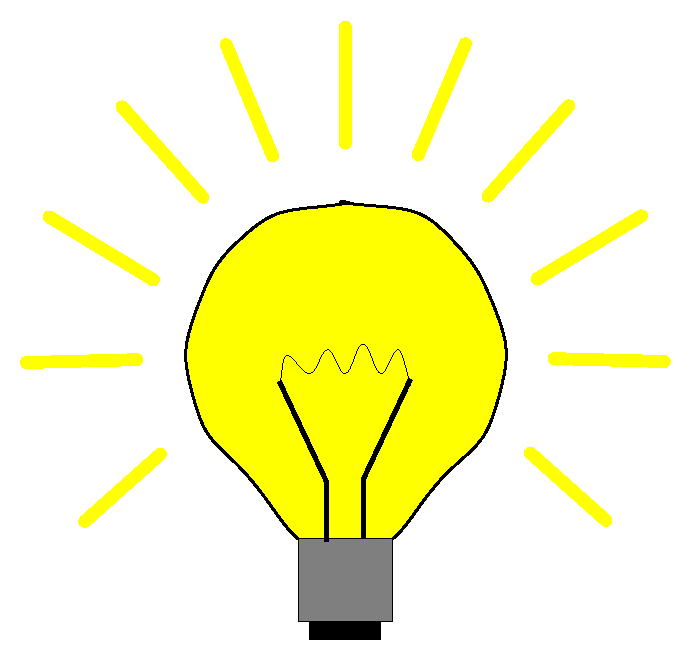
\includegraphics[width=0.7cm]{figures/tip.eps}}]%
          {{\vspace{0.1cm}\hspace{-0.2cm}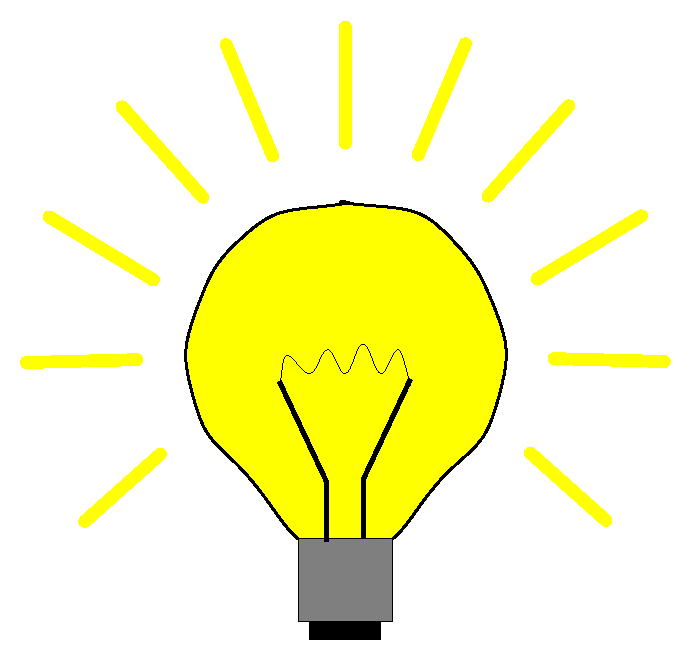
\includegraphics[width=0.7cm]{figures/tip.eps}}}%
\hspace{0.5cm}\psframebox*[fillcolor=tipbg]{\parbox{\NoteBoxWidth}{#1}}\vspace*{0.4cm}}

\newcommand{\NOTE}[1]{\vspace*{0.4cm}
\marginpar[{\vspace{0.15cm}\hspace{ 0.8cm}
\includegraphics[width=0.7cm]{figures/note.eps}}]%
          {{\vspace{0.15cm}\hspace{-0.2cm}
\includegraphics[width=0.7cm]{figures/note.eps}}}%
\hspace{0.5cm}\psframebox*[fillcolor=notebg]{\parbox{\NoteBoxWidth}{#1}}\vspace*{0.4cm}}

\newcommand{\listitem} {\psframe[fillstyle=gradient,gradbegin=headingfg,gradend=headingfg,gradmidpoint=1,linestyle=none](-0.15,0.075)(0.0,0.225)}

\newenvironment{mmnttable}[3]
{\renewcommand{\mmntcaparg}{#3}\par\vspace{3mm}\begin{minipage}{\textwidth}
\begin{center}\par\begin{tabular}{#1} \hline #2 \\ \hline}
{\hline \end{tabular}\mmnttablecaption{\mmntcaparg}\end{center}\end{minipage}}
\makeatother

\newenvironment{exaipd}
{ %\begin{list}{}{\leftmargin6mm} \scriptsize\item[]\EXA }
 \begin{list}{}{\leftmargin6mm} \scriptsize\item[]\EXA }
{\end{list}}

\newenvironment{mmnttableL}[4]
{\renewcommand{\mmntcaparg}{#3}\renewcommand{\mmntlabarg}{#4}\par
\vspace{3mm}\begin{minipage}{\textwidth}\begin{center}\par\begin{tabular}{#1}
\hline #2 \\ \hline}
{\hline \end{tabular}\mmnttablecaption{\mmntcaparg}\label{\mmntlabarg}
\end{center}\end{minipage}}

\newenvironment{mmntlist}
{\par\vspace*{-0.1cm}%
  \begin{list}{\listitem}%
      {\setlength{\itemsep}{0.001cm}}%
}%
{\end{list}\vspace*{-0.1cm}}

